\chapter{The Large Hadron Collider and ATLAS experiment}
\label{chap::LHC}

\chapterquote{Bigger...}%
{Everyone when I ask them about the FCC}

\section{The Large Hadron Collider}
In order to probes the fundamentals of the universe we have to build a particle accelerator powerful enough to reach high enough energies to recreate the conditions moments after the big bang. Enter the Large Hadron Collider (LHC). LHC straddles the Swiss-French border, near the city of Geneva. It is a hadron accelerator, delivering proton-proton collisions and also supporting collisions of protons with heavy ions or simply just heavy ion collisions. The LHC sits in a tunnel with a circumference of 27 Km, the tunnel varies in depth sitting between 40 m to 120 m below the surface. The LHC is designed to operate at a cernt of mass energy of $\sqrt{s}=14$ TeV with an instantaneous luminosity of $L=10^{34}\text{cm}^{-2}\text{s}^{-1}$. The LHC collides beams of accelerated charged particles traveling in opposite directions inside two separate rings which each contain a vacuum. The Beams are deflected by supper conducting magnets keeping them centered in the rings. The beams are collide at four focus points around the LHC 'ring' where the major experiments are positioned, these experiments are: ATLAS \refs, LHCb\refs, CMS\refs and ALICE\refs.



\subsection{The CERN accelerator chain}
The LHC is fed by a series of particle accelerators deigned to take ionized hydrogen gas and accelerate the protons before they reach the LHC. The chain of accelerator are as follows:  First we begin with a bottle of Hydrogen gas, the electrons are then stripped from the hydrogen, ionizing it resulting in raw protons. These protons are then accelerated up to an energy of 50MeV in the LINear ACcelerator 2 (LINAC2)\textcolor{red}{refs}. It is then fed into the Proton Synchrotron booster (PSB) \textcolor{red}{refs} and accelerated to 1.4GeV and subsequently to 450 GeV by the Proton Synchrotron (PS)\textcolor{red}{refs}. At this point the proton beam is split into two and enter the LHC in a clockwise and anti-clock wise direction. Once in the LHC the proton beams should ideally reach an energy of 7 TeV each, resulting in an ideal center of mass energy of $\sqrt{s}=14$TeV. A detailed layout of the accelerator network can be found in Figure\ref{fig:CERN-acc}.
\begin{figure}[h!]
    \centering
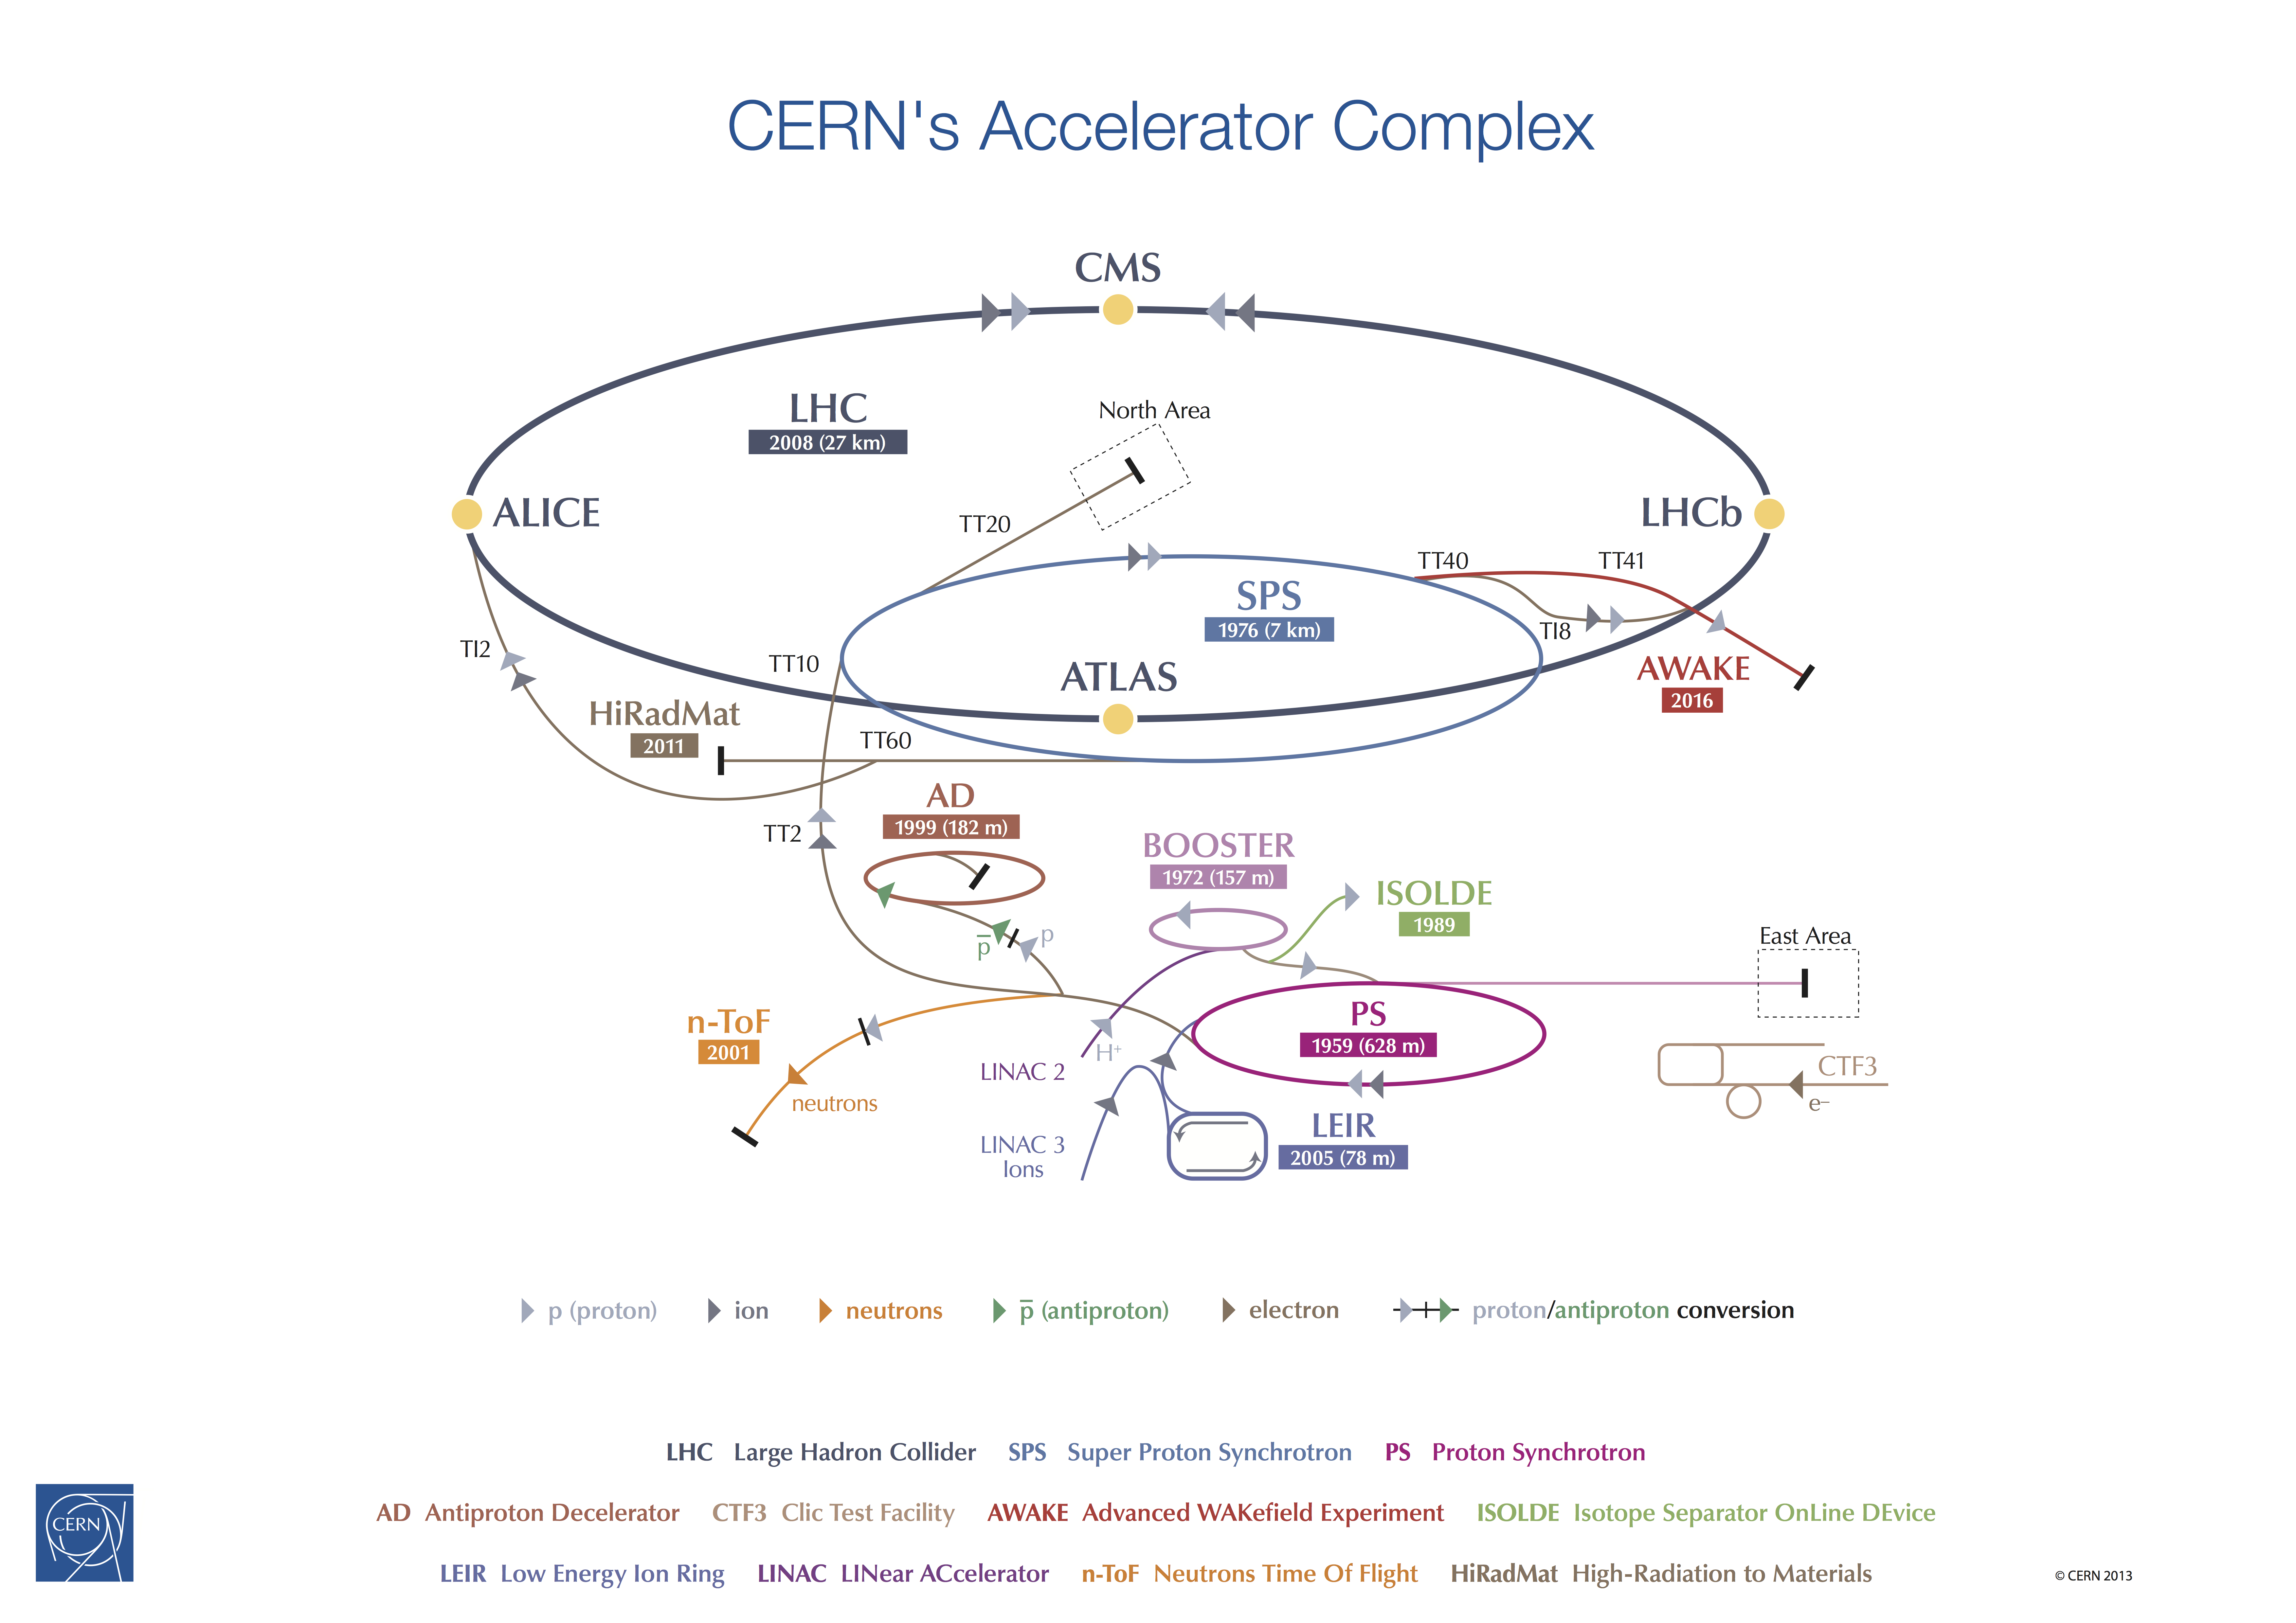
\includegraphics[scale=0.14]{Section_ATLAS_dect/LHC-complex.jpg}
    \caption{A summary diagram of the CERN accelerator network.\textcolor{red}{refs}}
    \label{fig:CERN-acc}
\end{figure}
\\
\\
This these will focus on the data taken during, the 2015-2018 data taking period, or Run-2. During this period the center of mass energy peaked at $\sqrt{s}=13$TeV. After the completion of Run-2, the LHC accelerator chain has seen a number of upgrades, the main of which is the introduction of LINAC4 \refs, which replaces the now decommissioned LINAC2 and the increase of LHC center of mass energy to $\sqrt{s}=13.6$TeV. LINAC4 is designed to accelerate negative hydrogen ions then stripping the ions of all electrons upon its exit and into the next accelerator in the chain. 

\subsection{Luminosity and pile-up}
As we discussed, the LHC mainly accelerates protons and thus produces proton-proton collisions we call these collisions events. The number of events, $N_{\text{events}}$, produced by the LHC as a function of instantaneous luminosity as a function of time, $t$, is given by\refs:
\begin{equation}
    N_{\text{events}} = \sigma_{\text{event}}\int L dt = \sigma_{\text{event}} \mathcal{L},
\end{equation}
where $\sigma_{\text{event}}$ is the cross-section of your given event and $\mathcal{L}$ is the integrated luminosity. We define the instantaneous luminosity as: 
\begin{equation}
    L=f\frac{n_1 n_2 }{4\pi \sigma_x \sigma_y}N_b.
\end{equation}
The nominal spacing between bunches is 25ns, with a collision frequency of $f=40$MHz. the number of protons per bunch is denoted by $n_1,n_2$ (one for each direction of travel of the beams) and $N_b$ is the number of bunches. The height and width of the Gaussian beam profile is given by $\sigma_x$ and $\sigma_y$, respectively. The integrated luminosity is used to quantity the volume of data that is collected over a give period of time.
\\
\\
Due to the large number of protons per bunch, one would assume that more than one hard scattering interaction takes place per bunch crossing. Interactions beside the interaction of interest is called pile-up, there are two kinds of pile-up: in-time and out-time pile-up. We define in-time pile-up as when there are more then one radiation event arrives at a detector simultaneously or very close together in time. This is usually caused by bunch crossings at the central point of collisions. Bunch crossings that result in an extra interaction but occur past the central crossing point, resulting in a radiation event arriving at the detector much later resulting in this event not being recorded properly or not being recorded at all. 

\section{The ATLAS detector}
The ATLAS Detector is a general purpose detector, meaning that it conducts a broad range of high energy particle physics analyses are conducted with ATLAS, including measurements of SM properties and searches for hints of BSM physics. The ATLAS detector is also the largest of the major particle physics detector experiments based at CERN. It measures 44m in length with a 25m diameter and weighs in at a slim 7,000 tonnes. The LHC beampipe travels along the center of the cylindrical detector with proton-proton collisions occurring at the, rough, geometric center of the detector. The detector is designed in layers of sub-detectors, with each layer designed to detect and record different types of particles.
\\
\\
The First layers begins 3 cm away from the beam pipe, this layer is designed to log the tracks of the charged particles produced immediately after the a proton-proton collision. These charged particles then hit layers designed to measure the electromagnetic and hadronic showers produced using dedicated calorimeters for each. Finally the outer most layers of the ATLAS detector is designed to make precision measurements of the muons produced after the proton-proton collisions. Along with the layers of silicon that make the sub-detectors there are also two systems of super conducting magnets, to provide magnetic fields for the tracking sub-detectors. The overall detector subsystems are split up into a barrel and two end cap regions providing almost full $4\pi$ coverage. 
\begin{figure}[h!]
    \centering
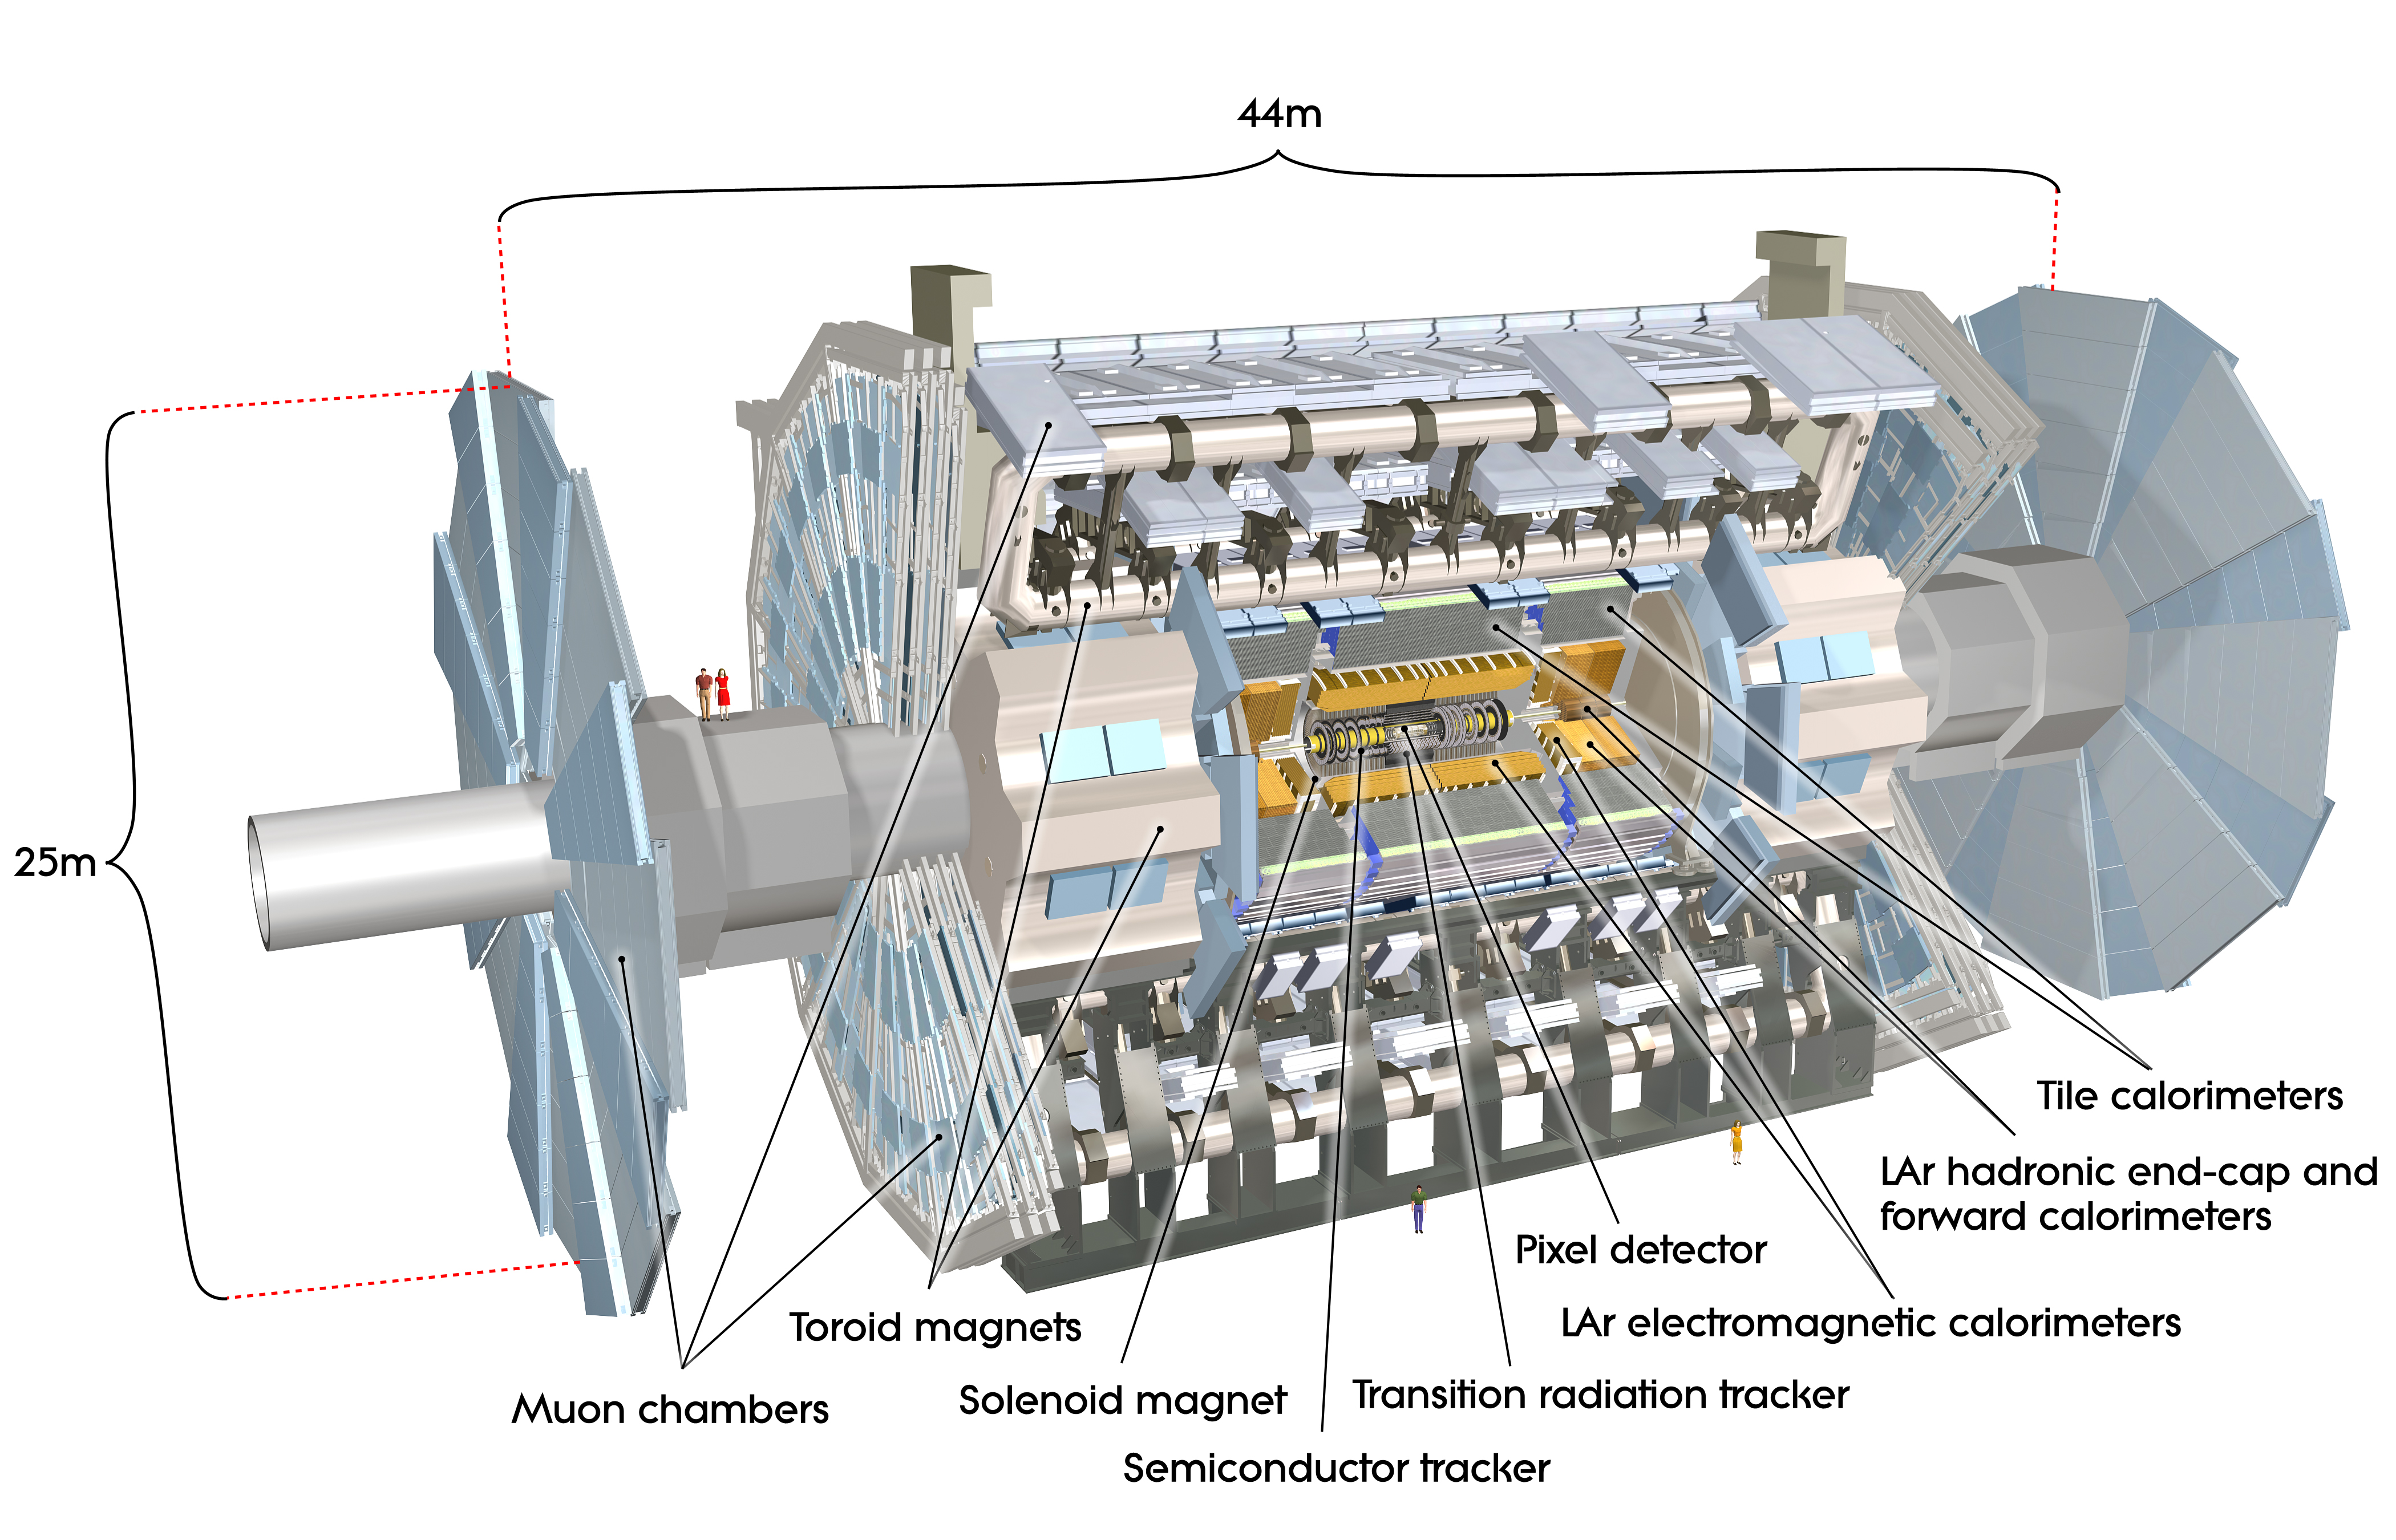
\includegraphics[scale=0.14]{Section_ATLAS_dect/full_detector.jpg}
    \caption{ Computer generated image of the whole ATLAS detector, identifying different parts of the detector and two people are shown for scale \cite{Pequenao:1095924}. \textcolor{red}{refs}}
    \label{fig:CERN-acc}
\end{figure}
\subsection{Coordinate systems}
Given the cylindrical shape of the ATLAS detector, we use both, a right-handed Cartesian coordinate system $(x,y,z)$ and cylindrical polar coordinates $(r,\theta,\phi)$. The interaction point, which is defined as the geometrical center of the detector and the origin of the coordinate systems. The positive $x$-direction of the defined Cartesian coordinates, points towards the center of the LHC ring. The positive $y$-direction points upwards. The $z$-direction is a tangent to the LHC beam pipe and is positive in the counter-clock wise direction of the beam pipe.
\\
\\
Using the cylindrical polar coordinates, $r$ is the distance from the beam line. The azimuthal angle, $\phi$ is the angle around the $z$-axis and has a $[\pi,-\pi]$ range. The polar angle $\theta$ is measured in the (x,z) plane and is the angle from the positive $z$-axis.
\\
\\
As we collide particle in the $z$-direction we use variables which are Lorentz invariant in this direction. We define the transverse momentum of a particle as $p_T = \sqrt{p_x^2 + p_y^2},$ this is an invariant quantity under boosts along the $z$-axis. The longitudinal momentum, $p_z$, however, changes unders such boosts and is therefore replaced with rapidity, which is defined as:  
\begin{equation}
    y=\frac{1}{2}\ln\left(\frac{E+p_z}{E-p_z} \right),
\end{equation}
where E is the energy of a particle. Rapidity its self is not Lorentz invariant but the difference in rapidity are invariant under boosts along the $z$-direction. if we consider a highly energetic massless particles, $E\gg m$, rapidity reduces to pseudorapidity, which gives us a Lorentz invariant quantity measure of $\theta$:
\begin{equation}
    \eta =-\ln\left( \tan\frac{\theta}{2}\right).
\end{equation}
Pseudorapidity approaches infinity as the
polar angle decreases to zero. Using this set of coordinates and variables we can define the distance between two objects in the $(\eta, \phi)$ plane as:
\begin{equation}
    \Delta R = \sqrt{(\Delta \eta)^2 + (\Delta\phi)^2}.
\end{equation}
\subsection{Magnet system}
the ATLAS detector has two superconducting magnet systems\refs: the first system is a central solenoid magnet which creates a 2T magnetic field for the inner tracking detector. the second system uses a series of tariodal magnets to create magnetic fields for the outer muon tracker (1T), one for each endcap region, and the barrel region (0.5T). The two magnet systems are shown on Figure \ref{fig:magsystem}.
\begin{figure}[h!]
    \centering
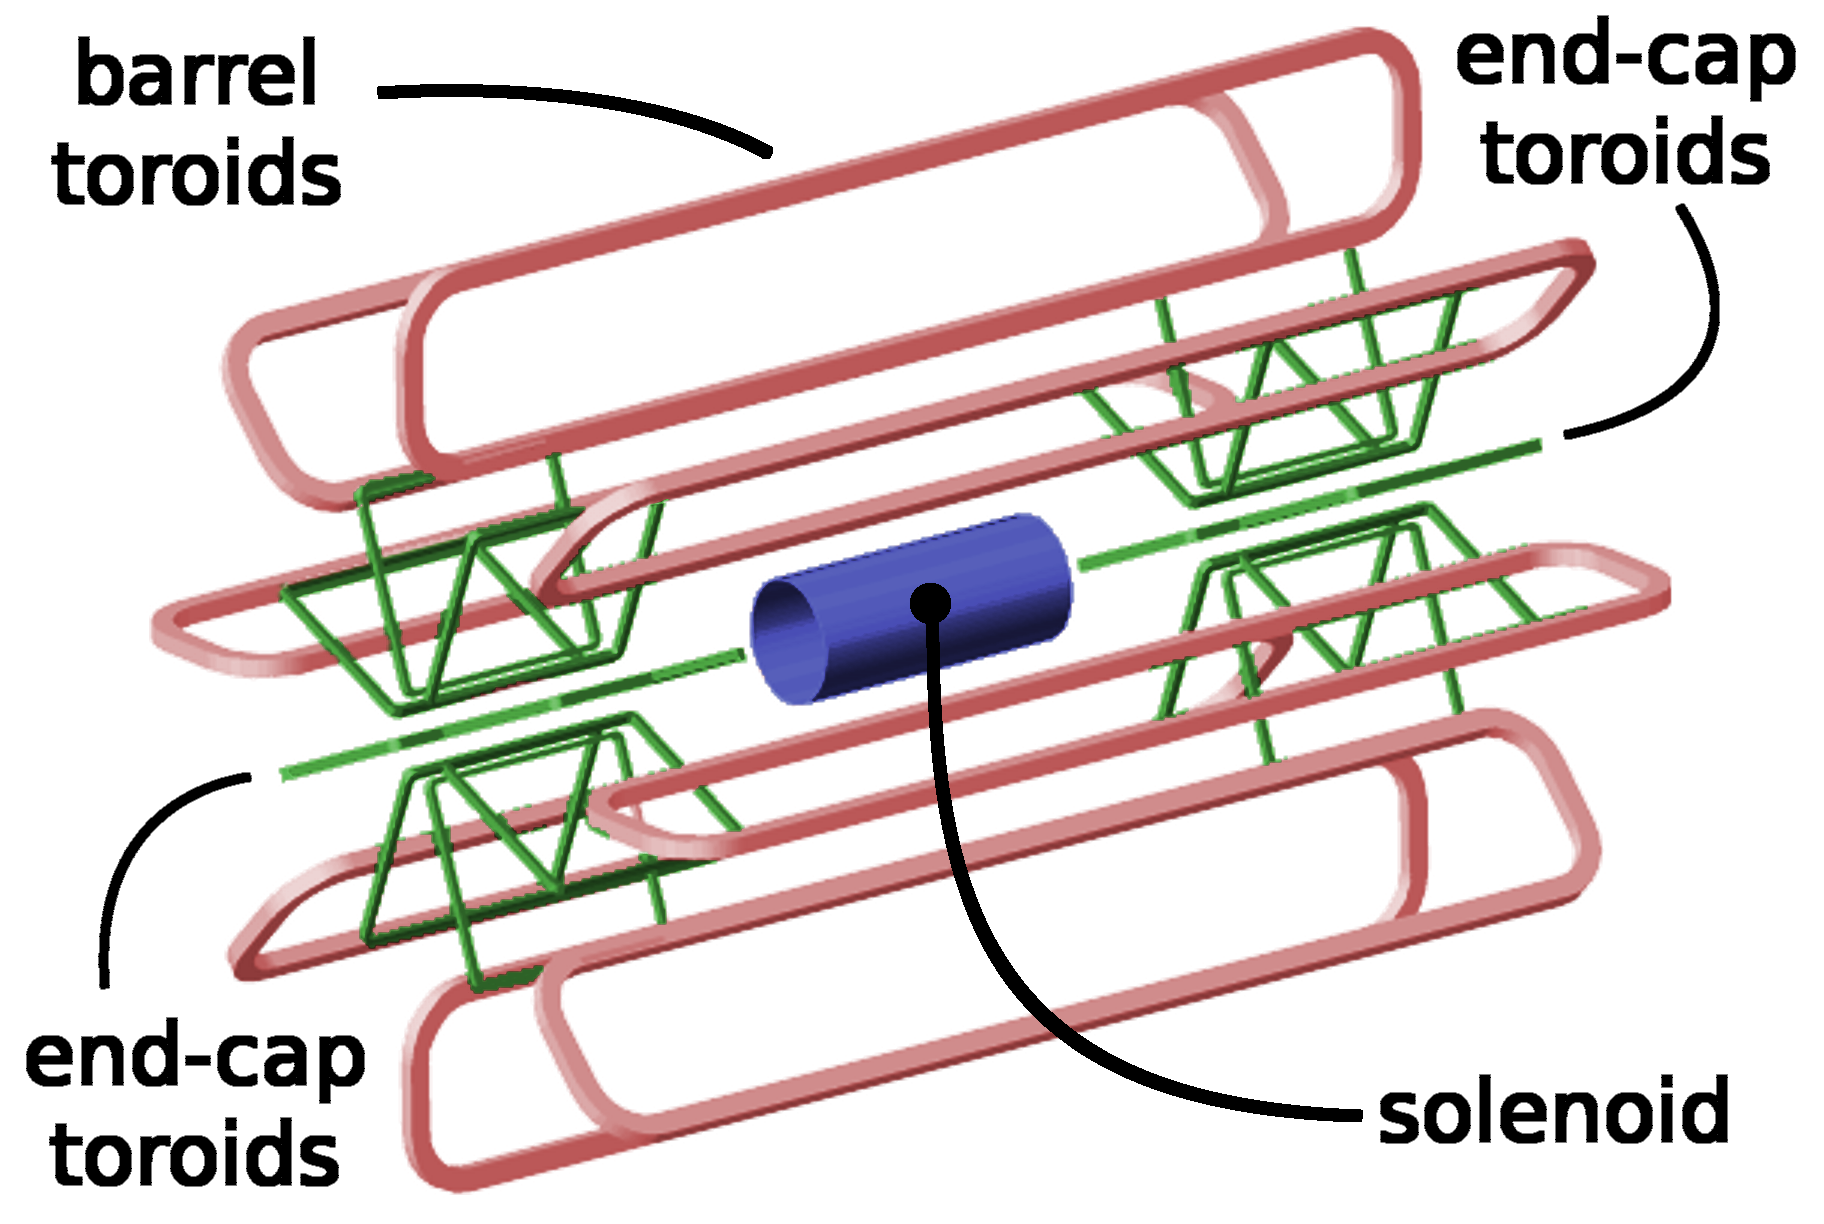
\includegraphics[scale=0.14]{Section_ATLAS_dect/magnetSystems.png}
    \caption{Computer generated image of the ATLAS magnet system \cite{magnets}. \textcolor{red}{refs}}
    \label{fig:magsystem}
\end{figure}
\subsection{Inner detector}
The Inner Detector \refs is the section of the detector closets to the beam pipe. It is designed to register a series of points, or \textit{hits}, along the path of a passing charged particle. These hits left by the particles are used to reconstruct the path, or track, of the particle. using the magnetic field of the central solenoid magnet, the ID is able to record the direction and curvature of each track allowing it to determine the momentum and charge of the particle. The ID is split up into three main regions: The pixel detector, which sits at the innermost layer of the ID, the semiconductor tracker, and finally, the Transition radiation tracker.
\subsubsection{Pixel detector}
The Pixel Detector \refs is the first point of contact for particles post collision. It is made up of four layers of silicon pixel sensors in the barrel region and three layers in the endcap regions. When the charged particles are incident on the silicon, electro-hole pairs are created which generate an electronic signal, this is then readout and recorded. The layer closest to the beam pipe is the Insertable B-Layer (IBL) \refs, this is designed to improve the identification of secondary vertices associated with B-hadron decays, improving the quality of data from the remaining pixel layers. The IBL has the finest pixels with a size of $50\times250 \,\text{\textmu m}^2$ while the remaining pixel layers have a size of $50\times400 \, \text{\textmu m}^2$. There are a total of 92 million pixels which cover a total of 1.9 $\text{m}^2$, a full azimuthal angle and $|\eta|<3$. It achieves a resolution of 10 \textmu m in the orthogonal direction of the beam pipe and a resolution of 115 \textmu m parallel to the beam pipe.
\subsubsection{Semi-conductor tracker}
The Semi-Conductor Tracker (SCT) \refs is the main layer of the ID and surrounds the pixel detector with modules of long silicon strip sensors. The SCT modules are arranged in four layers in the barrel region ($|\eta|<1.4$) and nine planar layers discs in the endcap regions ($1.4<|\eta|<2.5$). Each module contains two silicon strip sensors placed at a slight offset in order to improve the spatial resolution. In total, the SCT contains 4,088 modules of double sided silicon strips resulting of 60$\text{m}^2$ of silicon. The SCT has a resolution of 17 \textmu m in the ($r-\phi$) plane and 580 \textmu m in the $z$-direction.
\subsubsection{Transition Radiation Tracker}
The Transition Radiation Tracker (TRT) \refs is the final and largest layer of the ID, its used for particle tracking and pion-electron separation. The TRT is constructed using two main components: drift tubes with a diameter of 4 mm, filled with a mixture of Xe, $\text{O}_2$ and $\text{CO}_2$ gases, and gold-plated tungsten wire with a diameter of 30 \textmu m which is stretched along the length of the tube. As a charged particle enters the drift tube, the gas is then ionised releasing electrons from the gas. These electrons then drift towards the anode wire creating a signal. The drift tubes are arranged in 73 barrel layers and 122 layers in each endcap giving an average of 30–40 position measurements per track. The TRT is also able to track particle in the $|\eta| < 2$ region with a spatial resolution of 130 \textmu m in the ($r - \phi$) plane which is notably worse than is silicon-based counterparts. However, because of the unique construction of the TRT, it is able to provide bespoke information in aiding to the discrimination of pions and electrons due to the differences in the amount of transition radiation generated by these particles. The TRT also improves the tracking performance of the ID, particularly at high transverse momentum due to many position measurements\refs.
\begin{figure}[h!]
    \centering
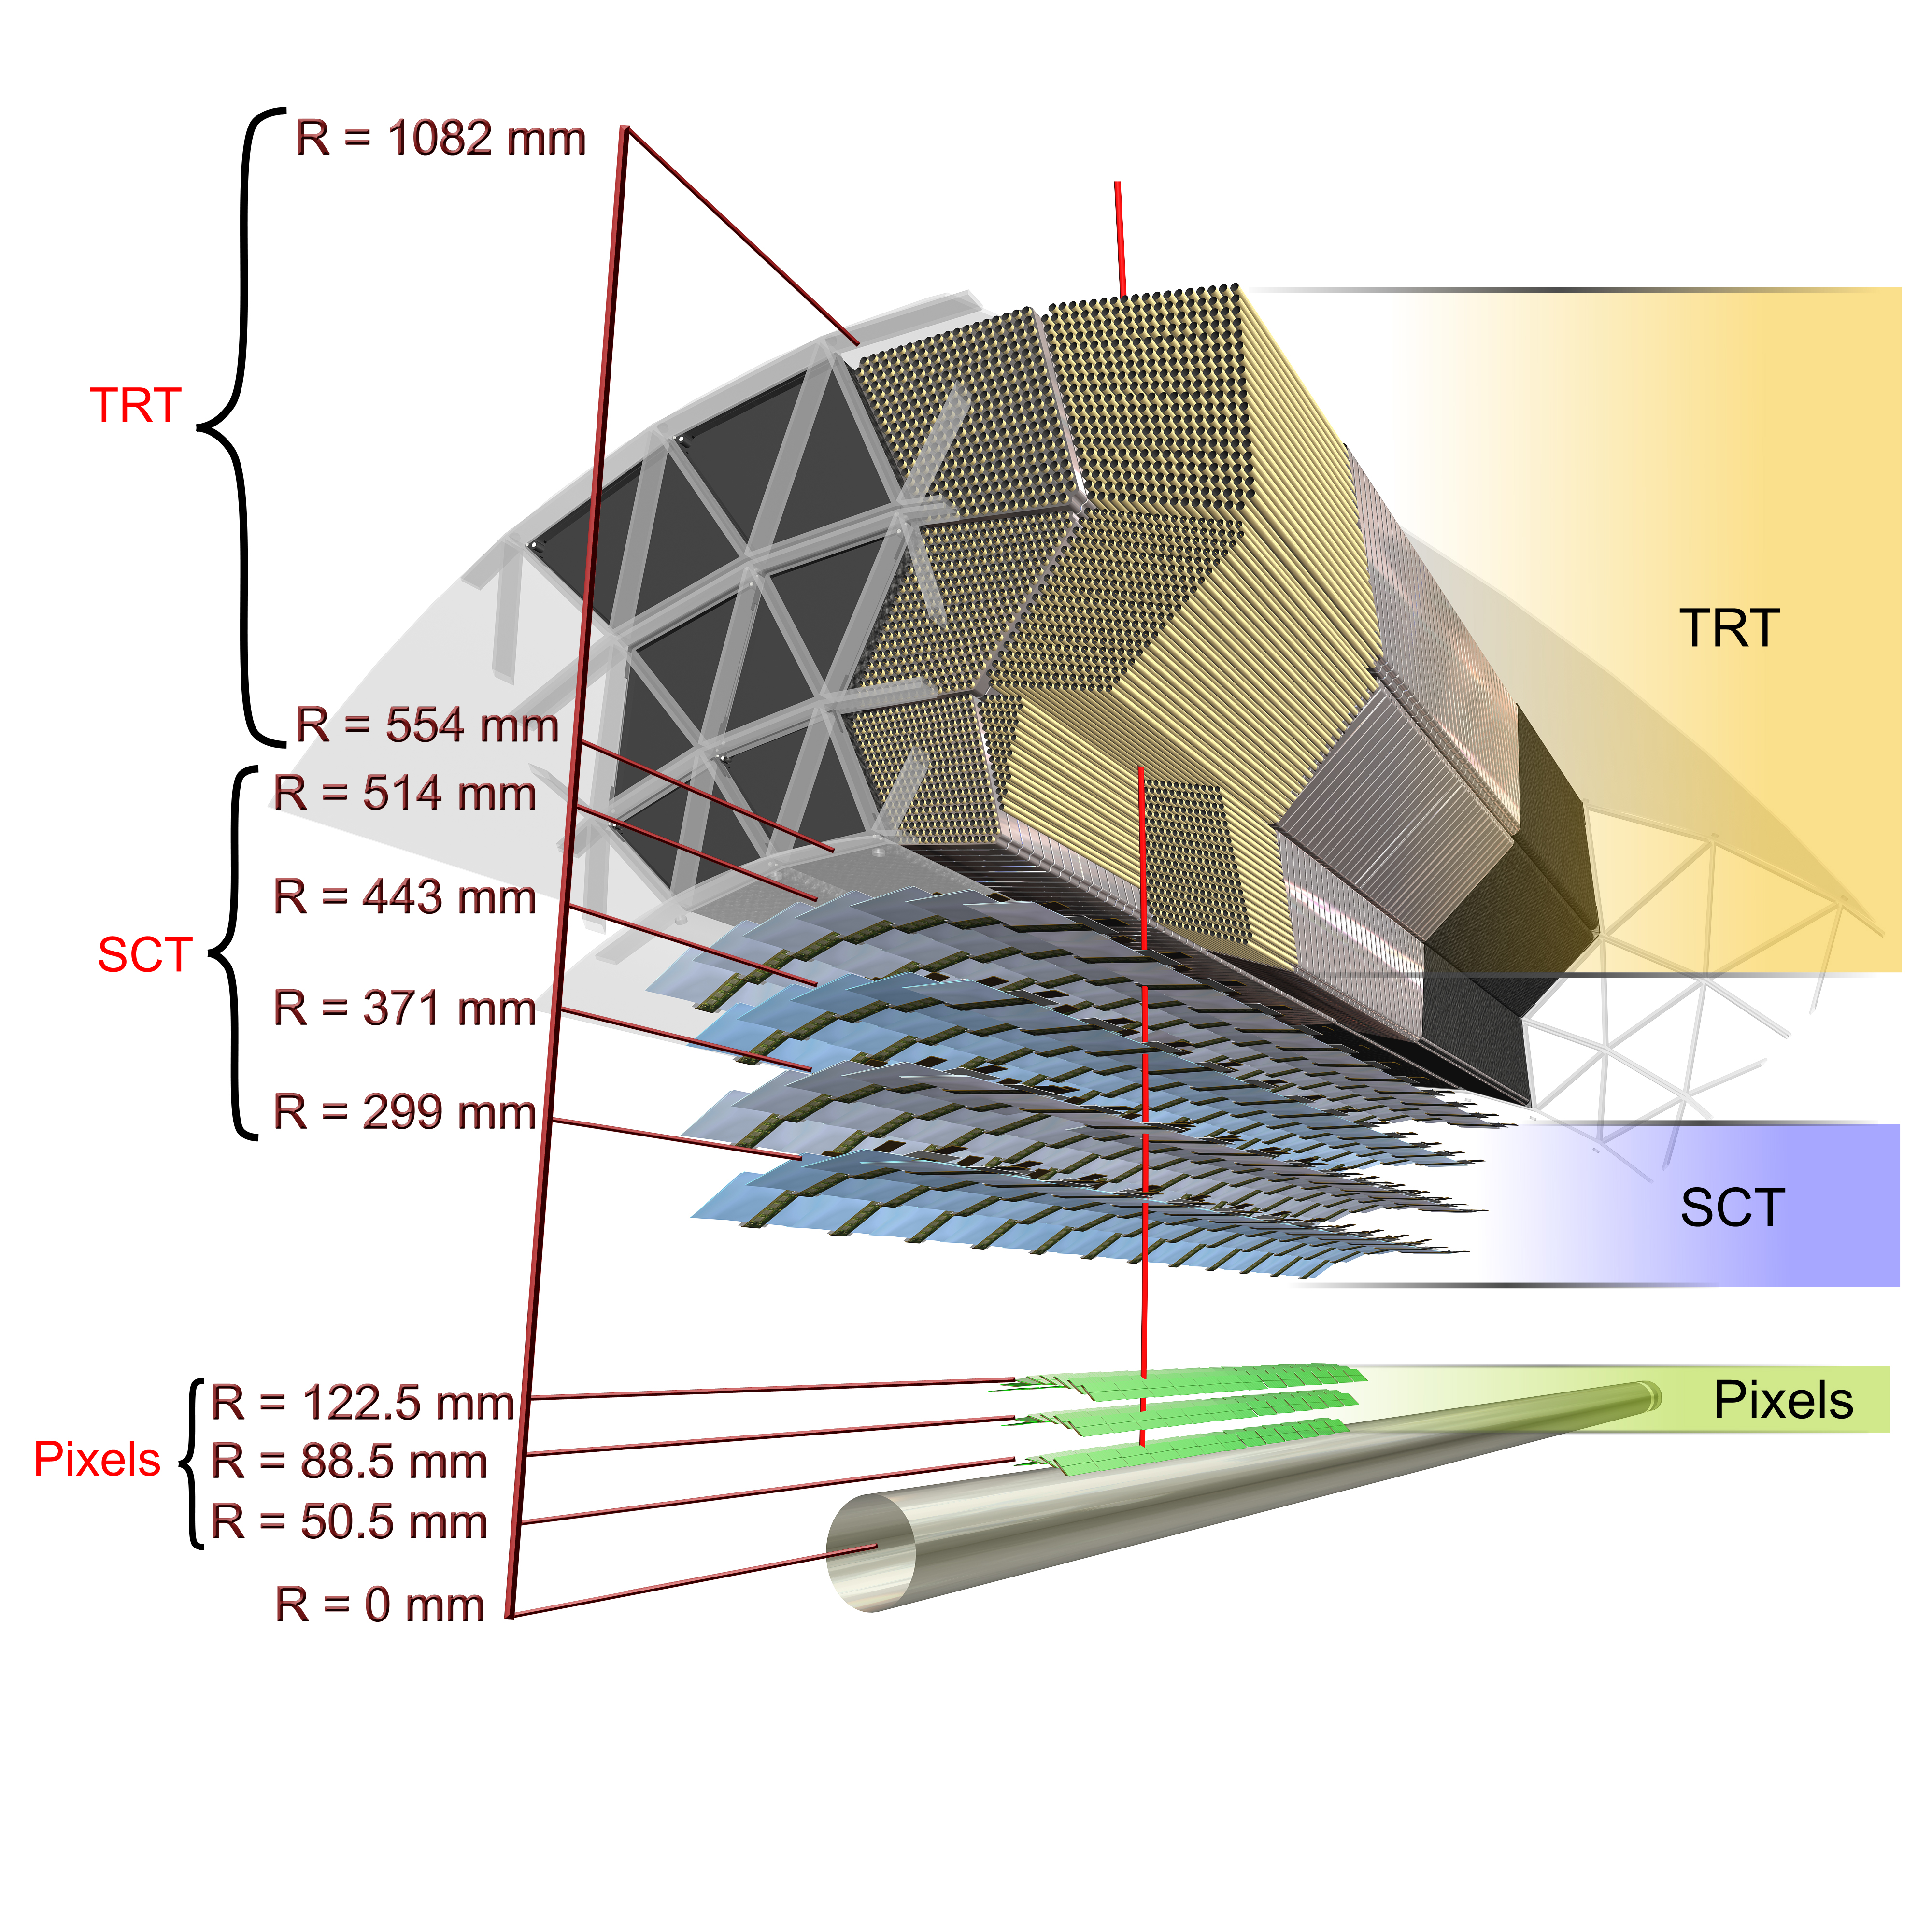
\includegraphics[scale=0.1]{Section_ATLAS_dect/tracker.jpg}
    \caption{Computer generated image of the ATLAS Inner Detector \cite{Pequenao:1095926tracker}.\textcolor{red}{refs}}
    \label{fig:CERN-acc}
\end{figure}
\subsection{Calorimeter}
After the ID, the next main set of layers in the ATLAS detector are the calorimeters. The ATLAS calorimeters \refs are designed to measure the energy of charged and neutral particles, namely, electrons, photons and hadrons. These calorimeteres are called sampling and are built in alternating layers of absorbing and active materials, nothing that the energy is only measured in the active layers. As high energy particles interact with these layers, they lose energy by producing cascades of secondary lower-energy particles, called showers. Electrons and photons lose energy with the material via electromagnetic interactions. Electrons above 10 MeV lose energy via bremsstrahlung, while photons undergo electron-positron production. The formation of hadronic showers is similar to that of electromagnetic cascades. 
\\
\\
There are two properties that is fundamental to the design of the calorimeter systems: the radiation length, $X_0$, which is a characteristic of a material, related to the energy loss of high energy particles electromagnetically interacting with it. And for hadronic interactions we consider the nuclear interaction length, $\lambda_I$, of a material. For a normal calorimeter material choice $\lambda_I >> X_0$. This means that electrons and photons interact much closer to the beam pipe than hadrons. So as a result, the ATLAS detector uses two calorimeters: and electromagnetic calorimeter and hadronic calorimeter. \textcolor{red}{pic of calirometer setup}

\subsubsection{Electromagnetic calorimeter}
The electromagnetic calorimeter (ECal) \refs uses liquid (LAr) in its active layers and lead (Pb) in its absorbing layers. The lead layers are designed to cause showering, the resulting particles then enter a LAr layer where ionisation occurs, resulting in electronic signals. The ECal is desgined to provide a consistent amount of material in all directions, corresponding to an interaction length of $22X_0$, covering a pseudo rapidity range of $|\eta| < 3.2$ and the full range of $\phi$. The Ecal is also split into the barrel region and endcap region. The barrel region starts with an active layer, called the pre-sampler. This is designed to measure the energy lost in the ID, after this there are then three finely granulated layers. In the endcap region there are only two, coarser, layers. \textcolor{red}{resolution of ECAL?}
\subsubsection{Hadronic calorimeter}
Follwoing the ECal we have the Hadronic Calorimeter (HCal). The HCal uses steel in the barrel region and copper in the endcap region, as the absorber layers, and scintillating tiles \refs in the barrel region and LAr in the endcap for the active layers. \textcolor{red}{resolution of HCal?}
\subsubsection{Forward calorimeter}
The Forward Calorimeter (FCal) is used to increase the precision of measuring missing transverse energy and naturally covers a higher range of pseudo-rapidity, $3.2<|\eta|<4.9$, compared to the barrel or endcap regions. The sampling is done using LAr for the active layers and copper and tungsten for absorbing layers. The FCal has three layers the first is designed to sample  electromagnetic showers and the other tow are designed to sample hadronic showers.  
\begin{figure}[h!]
    \centering
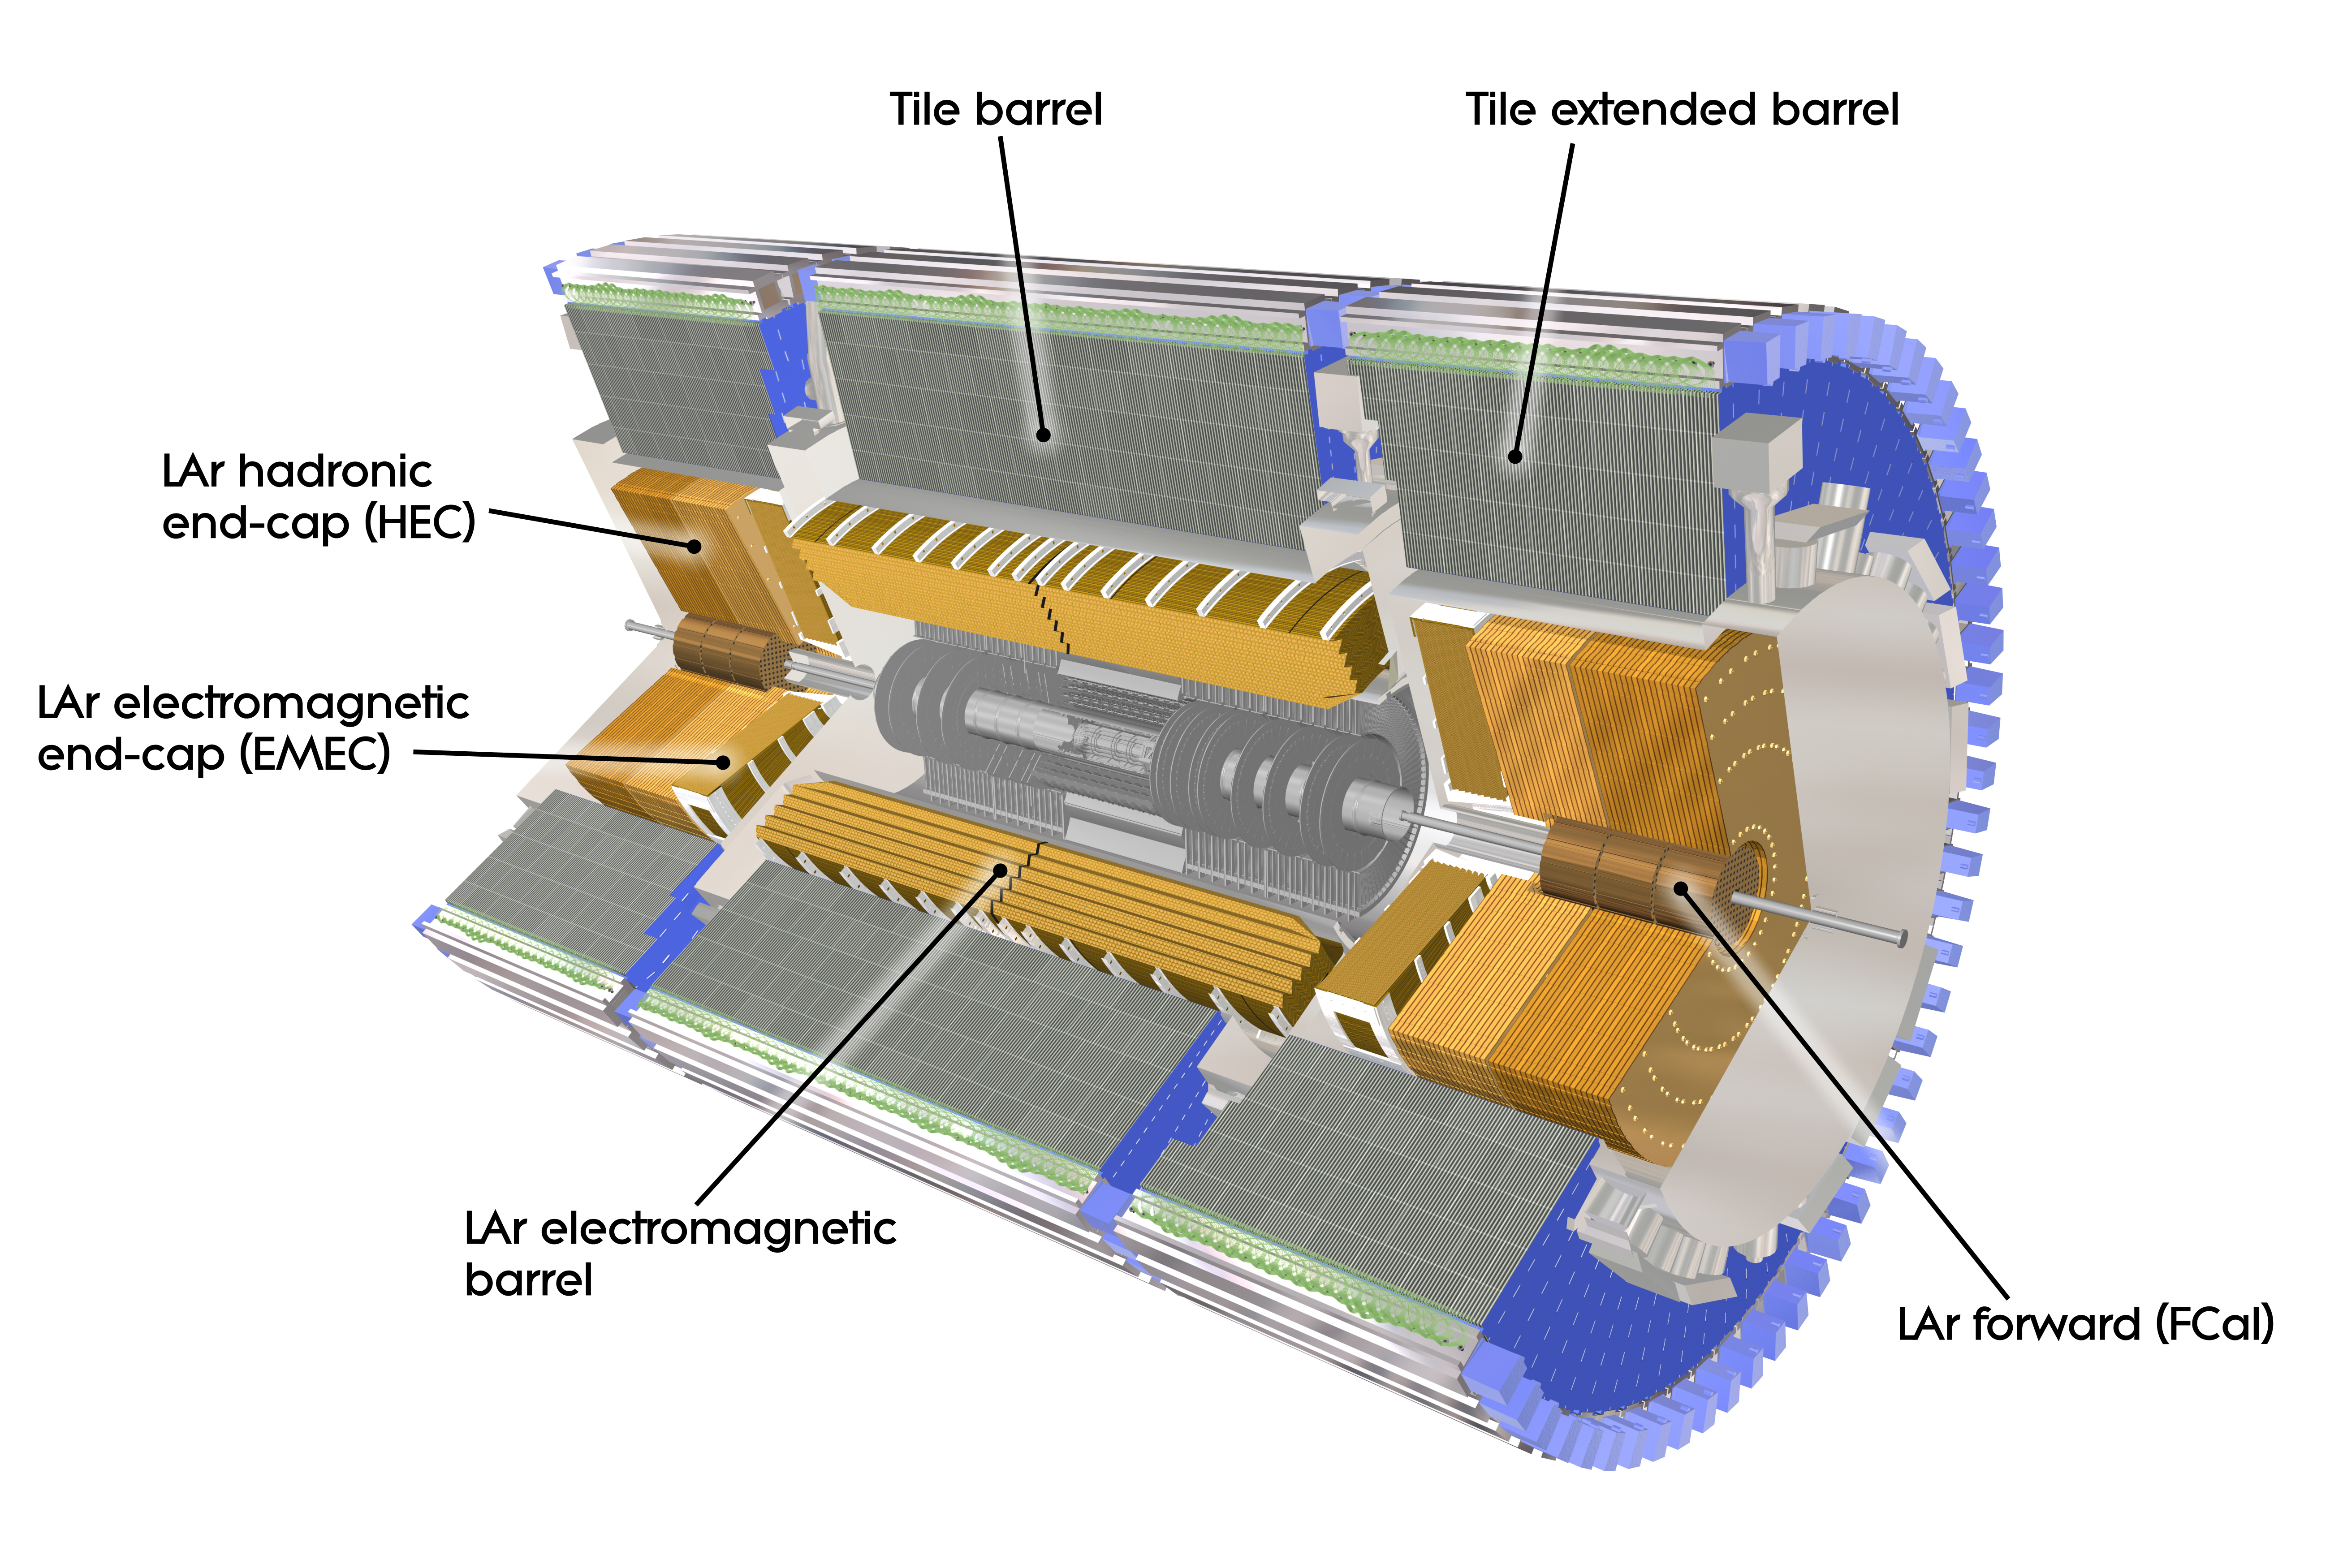
\includegraphics[scale=0.1]{Section_ATLAS_dect/cals.jpg}
    \caption{Computer generated image of the ATLAS calorimeters \cite{Pequenao:1095927cals}.\textcolor{red}{refs}}
    \label{fig:CERN-acc}
\end{figure}
\subsection{Muon spectrometer}

\subsubsection{Monitored drift tubes}

\subsubsection{cathode strip chambers}

\subsubsection{Resistive-plate chambers}

\subsubsection{Thin-gap chambers}

\section{Trigger and data acquisition systems}

\subsection{L1}
asdfadsfadadfadfadf
\subsection{High level trigger}
kfjdlgkj;adlfadskflj
\subsection{muon trigger}

\section{Future detector upgrades: The ITk}

